%From https://egu2018.eu/PICO_how-to_guide_to_PICO.pdf
%Abstracted and templated by Brian Ballsun-Stanton, Macquarie University.
%original template by https://github.com/snowtechblog/pico-latex-presentation by Anselm Köhler

\documentclass[unknownkeysallowed,usepdftitle=false, parskip=full]{beamer}
% unknownkeysallowed is needed for mac and the newer latex version -> is more picky than before...
\usetheme[headheight=1cm,footheight=2cm]{boxes}
%\usetheme{default}


\usepackage{default}
\usepackage{graphicx}
%example pictures created via: http://lorempixel.com/1200/800/cats/Figure2/. Credit to http://lorempixel.com/images.php

\usepackage{epsfig}
\usepackage{siunitx}
\usepackage{color}
\usepackage{ifthen}
%usepackage{ragged2e}

\usepackage[T1]{fontenc}
\usepackage[utf8]{inputenc}
%https://tex.stackexchange.com/a/203804/5483

\usepackage[activate={true,nocompatibility},final,tracking=true,kerning=true,spacing=true,factor=1100,stretch=10,shrink=10]{microtype} % http://www.khirevich.com/latex/microtype/
\microtypecontext{spacing=nonfrench}

\usepackage{lipsum} % for dummy text only
\usepackage[UKenglish]{babel} %https://tex.stackexchange.com/a/27743 
\usepackage[pangram]{blindtext} % https://tex.stackexchange.com/a/48411

%\usepackage{parskip} % from https://tex.stackexchange.com/q/11622
%\setlength{\parskip}{12pt} 

%\setparsizes{\parindent}{12pt}{\parfillskip}

%\usepackage{etoolbox} % as per https://tex.stackexchange.com/a/24331
%\appto\chapterheadendvskip{\vspace{-1\parskip}}
%\setparsizes{\parindent}{50pt plus 20pt minus 30pt}{\parfillskip}

\setbeamertemplate{navigation symbols}{}%remove navigation symbols
\setbeamersize{text margin left=1cm,text margin right=1cm}

% some colors
\definecolor{grau}{gray}{.5}
\definecolor{slfcolor}{rgb}{0,0.6274,0.8353}
\definecolor{wslcolor}{rgb}{0,0.4,0.4}

% setup links
\hypersetup{%
	%linkbordercolor=green,%
	colorlinks=true,%
	pdfborderstyle={/S/U/W 0},%
	%pdfpagemode=FullScreen,%
	pdfstartpage=4%
	}

% setup some fonts
\setbeamerfont{title}{series=\bfseries, size=\small}
\setbeamerfont{author}{size*={5pt}{0pt}}
\setbeamerfont{institute}{size*={3pt}{0pt}}
\setbeamerfont{bodytext}{size=\scriptsize}
	
% Title setup	
\title{\LaTeX\,\,style package: focusframe}
\author{Billy Black \texttt{42920477}}
% add title in headbox
\setbeamertemplate{headline}
{\leavevmode
\begin{beamercolorbox}[width=1\paperwidth]{head title}
    \vspace{0.1cm}
  % LOGO
  \begin{columns}[t, totalwidth=\textwidth]
  \begin{column}[c]{1.05cm}
     %
\includegraphics[width=1cm]{figure/logo1.png}
  \end{column}
  % TITLE
   \begin{column}[c]{10.6cm}
    \centering \usebeamerfont{title} \vspace{0.1cm}\textcolor{slfcolor}{\inserttitle} \\
   \centering \usebeamerfont{author} \color[rgb]{0,0,0} \insertauthor \\
   \vspace{0.1cm}
   \centering \usebeamerfont{institute} \insertinstitute
  \end{column}
  % PICTURE
  \begin{column}[c]{1.15cm}
    \hspace{0.005cm}
    %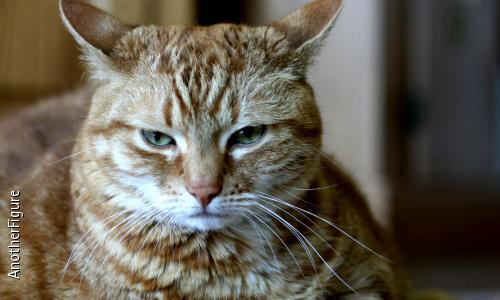
\includegraphics[width=1cm]{figure/figure1.png}
  \end{column}
  \end{columns}
  {\color{slfcolor}\hrule height 1pt\vspace{0.1cm}}
\end{beamercolorbox}%
}

% setup the navigation in footbox
% first set some button colors
\newcommand{\buttonactive}{\setbeamercolor{button}{bg=wslcolor,fg=white}}
\newcommand{\buttonpassive}{\setbeamercolor{button}{bg=slfcolor,fg=black}}
% now set up that the one active one gets the new color.
\newcommand{\secvariable}{nothing}
% therefore we write before each section (well, everything which should be part of the navi bar)
% the variable \secvariable to any name which is in the next function ...
\newcommand{\mysection}[1]{\renewcommand{\secvariable}{#1}
}
% ... compaired to strings in the following navibar definition ...
\newcommand{\tocbuttoncolor}[1]{%
 \ifthenelse{\equal{\secvariable}{#1}}{%
    \buttonactive}{%
    \buttonpassive}
 }
% ... here we start to set up the navibar. each entry is calling first the function \tocbuttoncolor with the argument which should be tested for beeing active. if active, then change color. afterwards the button is draw. so to change that, you need to change the argument in \toc..color, the first in \hyperlink and before each frames definition... A bit messed up, but works...
\newlength{\buttonspacingfootline}
\setlength{\buttonspacingfootline}{-0.2cm}
\setbeamertemplate{footline}
{\leavevmode
\begin{beamercolorbox}[width=1\paperwidth]{head title}
  {\color{slfcolor}\hrule height 1pt}
  \vspace{0.05cm}
  % set up the buttons in an mbox
  \centering \mbox{
    \tocbuttoncolor{abstract}
    \hyperlink{abstract}{\beamerbutton{2 Minute Madness}}
    \tocbuttoncolor{radar}
    \hspace{\buttonspacingfootline}
      \hyperlink{radar}{\beamerbutton{Alternatives}}

    \tocbuttoncolor{line}
    \hspace{\buttonspacingfootline}
      \hyperlink{line}{\beamerbutton{Chunking}}
    \tocbuttoncolor{major}
    \hspace{\buttonspacingfootline}
      \hyperlink{major}{\beamerbutton{Sectioning}}
    \tocbuttoncolor{slab}
    \hspace{\buttonspacingfootline}
      \hyperlink{slab}{\beamerbutton{Subsectioning}}
    \tocbuttoncolor{minor}
    \hspace{\buttonspacingfootline}
      \hyperlink{minor}{\beamerbutton{Demonstration}}
    \tocbuttoncolor{conclusion}
    \hspace{\buttonspacingfootline}
      \hyperlink{conclusion}{\beamerbutton{Links}}
    % this last one should normaly not be used... it will open the preferences to change the 
    % behaviour of the acrobat reader in fullscreen -> usefull in pico...
    \setbeamercolor{button}{bg=white,fg=black}
    % for presentation
    %\hspace{-0.1cm}\Acrobatmenu{FullScreenPrefs}{\beamerbutton{\#}}
    % for upload
    
     
\Acrobatmenu{FullScreenPrefs}{\vspace{0.3cm}\mbox{%
      
\includegraphics[height=0.04\textheight,keepaspectratio]{%
	  figure/CreativeCommons_Attribution_License.eps}%
	  }}
   }
    \vspace{0.05cm}
\end{beamercolorbox}%
}


\begin{document}


%%%%%%%%%%%%%%%%%%%%%%%%%%%%%%%%%%%%%%%%%%%%%%%%%%%%%%%%%%%%%%%%%%%%%%%%%%
\mysection{abstract}
%%%%%%%%%%%%%%%%%%%%%%%%%%%%%%%%%%%%%%%%%%%%%%%%%%%%%%%%%%%%%%%%%%%%%%%%%%
\begin{frame}\label{\secvariable}

\usebeamerfont{bodytext}


\parbox{\linewidth}{

\vspace{5pt}
%thesis
\textbf{You need to write 20 000 words for a research project. Where do you start?}



\vspace{12pt}
    \begin{columns}[t]
    %https://tex.stackexchange.com/a/7452/5483
    \begin{column}[c]{0.45\textwidth}
        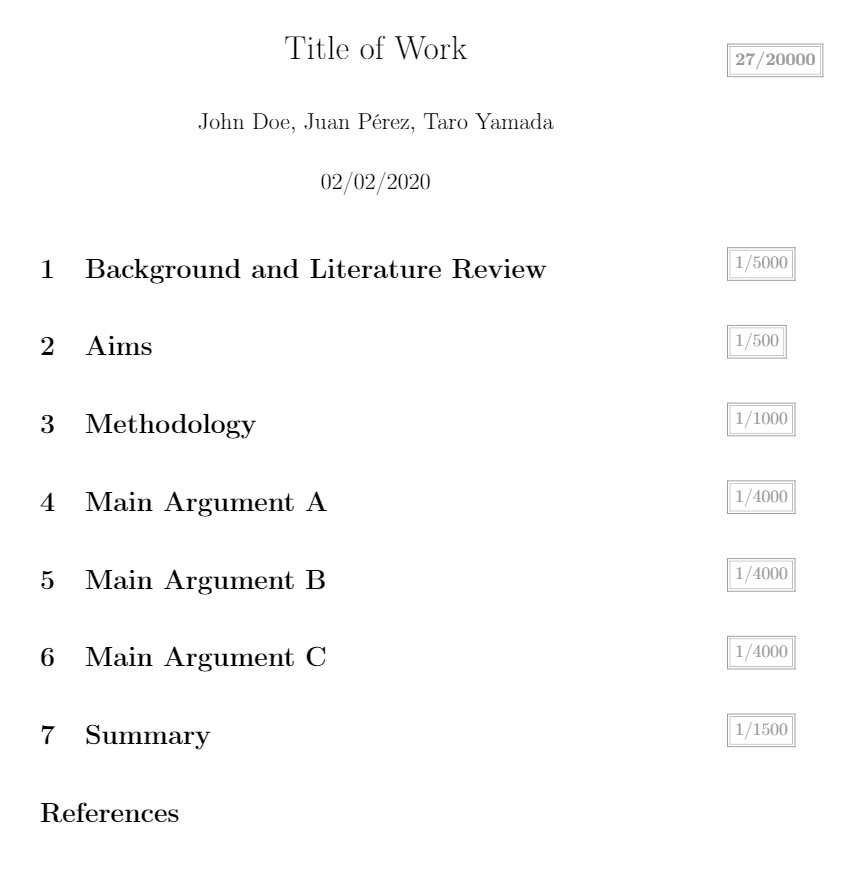
\includegraphics[scale=0.45]{figure/sectioning}
        \\
        \small Separating large documents into sections with word count goals.
    \end{column}
    \begin{column}[c]{0.45\textwidth}
    \parbox{\linewidth}{

    \small Separating sections into subsections with word count goals.
      
      \vspace{12pt}
      
    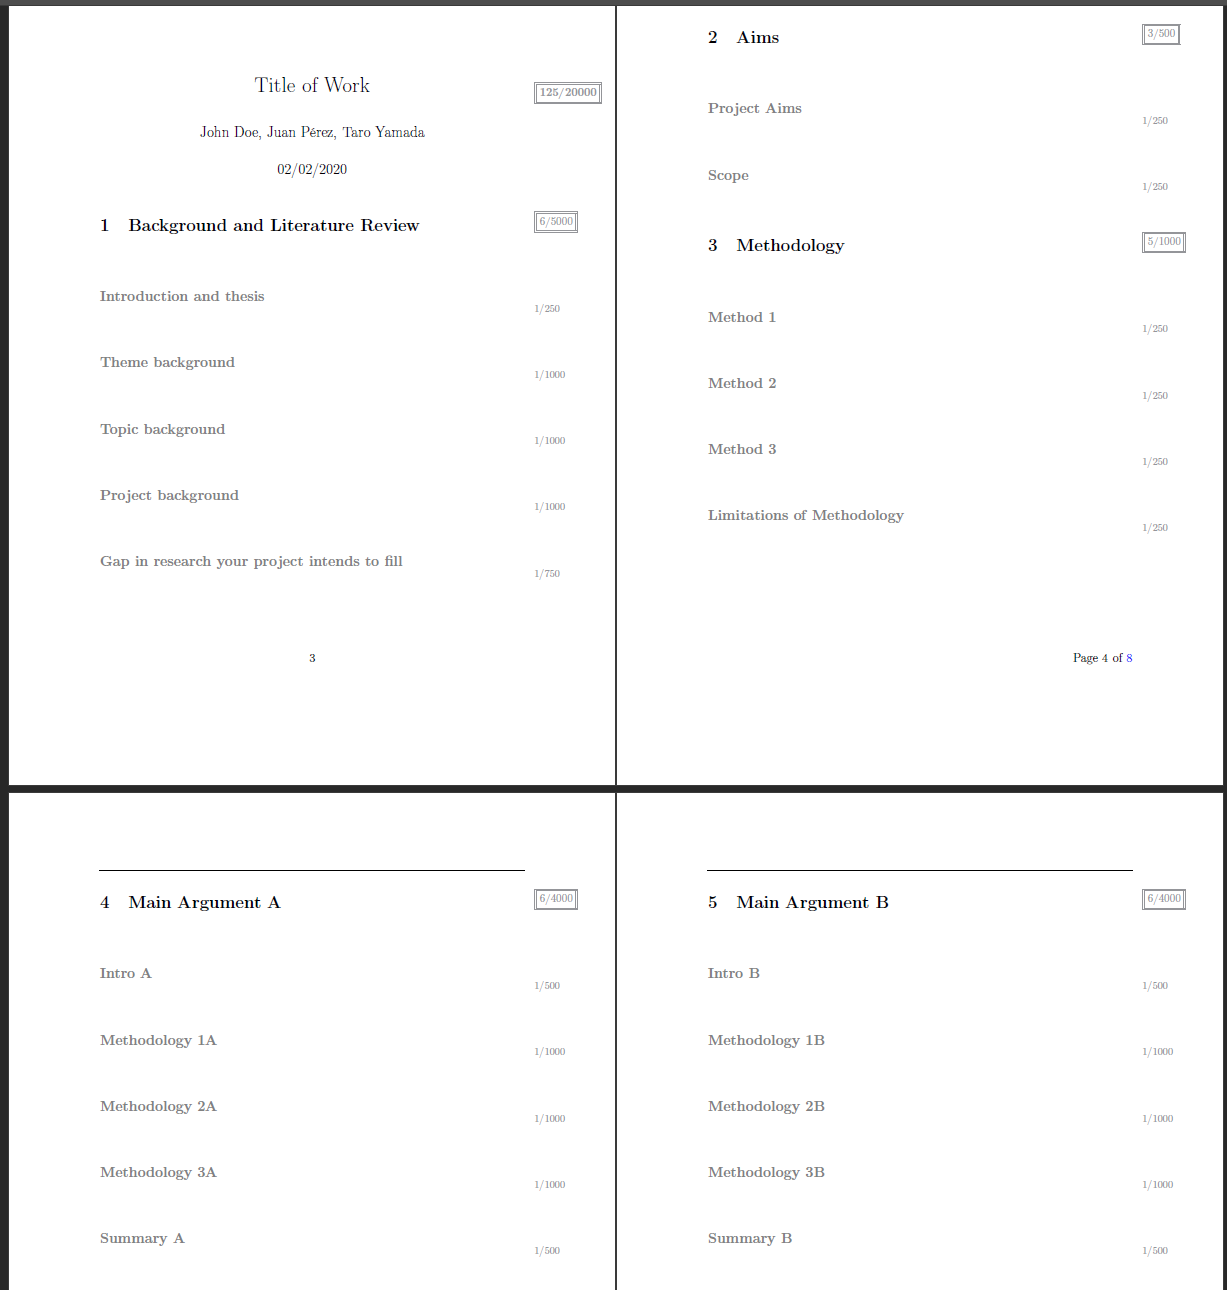
\includegraphics[scale=0.35]{figure/subsectioning}
      }
    \end{column}
    
  \end{columns}


}


   
\end{frame}

\begin{frame}\label{\secvariable}
\centering\includegraphics[scale=0.5]{figure/readmeeg.PNG}

\tiny{\textit{Screenshot of focusframe in action}}
  \scriptsize
  \begin{columns}[t]
  %https://tex.stackexchange.com/a/7452/5483
  \begin{column}[c]{0.6\textwidth}
    \begin{itemize}
        \vspace{-8pt}\item Free to run and does not require any copyrighted platform
        \item Costs less time to learn and implement than current simplest method of click-dragging and manually updating sections with word count
     \end{itemize}
    \end{column}
    \begin{column}[c]{0.6\textwidth}
    \parbox{\linewidth}{

    \begin{itemize}
        \item Can be toggled on and off to preview final version or for printing
        \item Visually represents colour-coded section progress without having to "read" and interpret numbers
            
        \end{itemize}
      }
    \end{column}
    
  \end{columns}
  
\end{frame}

%%%%%%%%%%%%%%%%%%%%%%%%%%%%%%%%%%%%%%%%%%%%%%%%%%%%%%%%%%%%%%%%%%%%%%%%%%
\mysection{radar}
%%%%%%%%%%%%%%%%%%%%%%%%%%%%%%%%%%%%%%%%%%%%%%%%%%%%%%%%%%%%%%%%%%%%%%%%%%
\begin{frame}\label{\secvariable}
  \begin{columns}[t]
  %https://tex.stackexchange.com/a/7452/5483
    \begin{column}[c]{0.45\textwidth}
    \parbox{\linewidth}{
\scriptsize
    \textbf{Drawbacks of the current alternative}
    
    \vspace{10pt}
      
      \begin{itemize}
          \item Highlighting text and manually editing counts takes time which adds up over the course of writing
          \item Manually editing counts breaks up flow of writing and can lead to distraction to look "neat"
          \item Typing counts manually interferes with formatting
          \item Cannot be temporarily removed or brought back
          \item When subsections are removed, previous subsection count becomes incorrect
          \item Full count undesirably includes bibliography
          \item Not legible when document is zoomed out
      \end{itemize}
      }
    \end{column}
    \begin{column}[c]{0.6\textwidth}
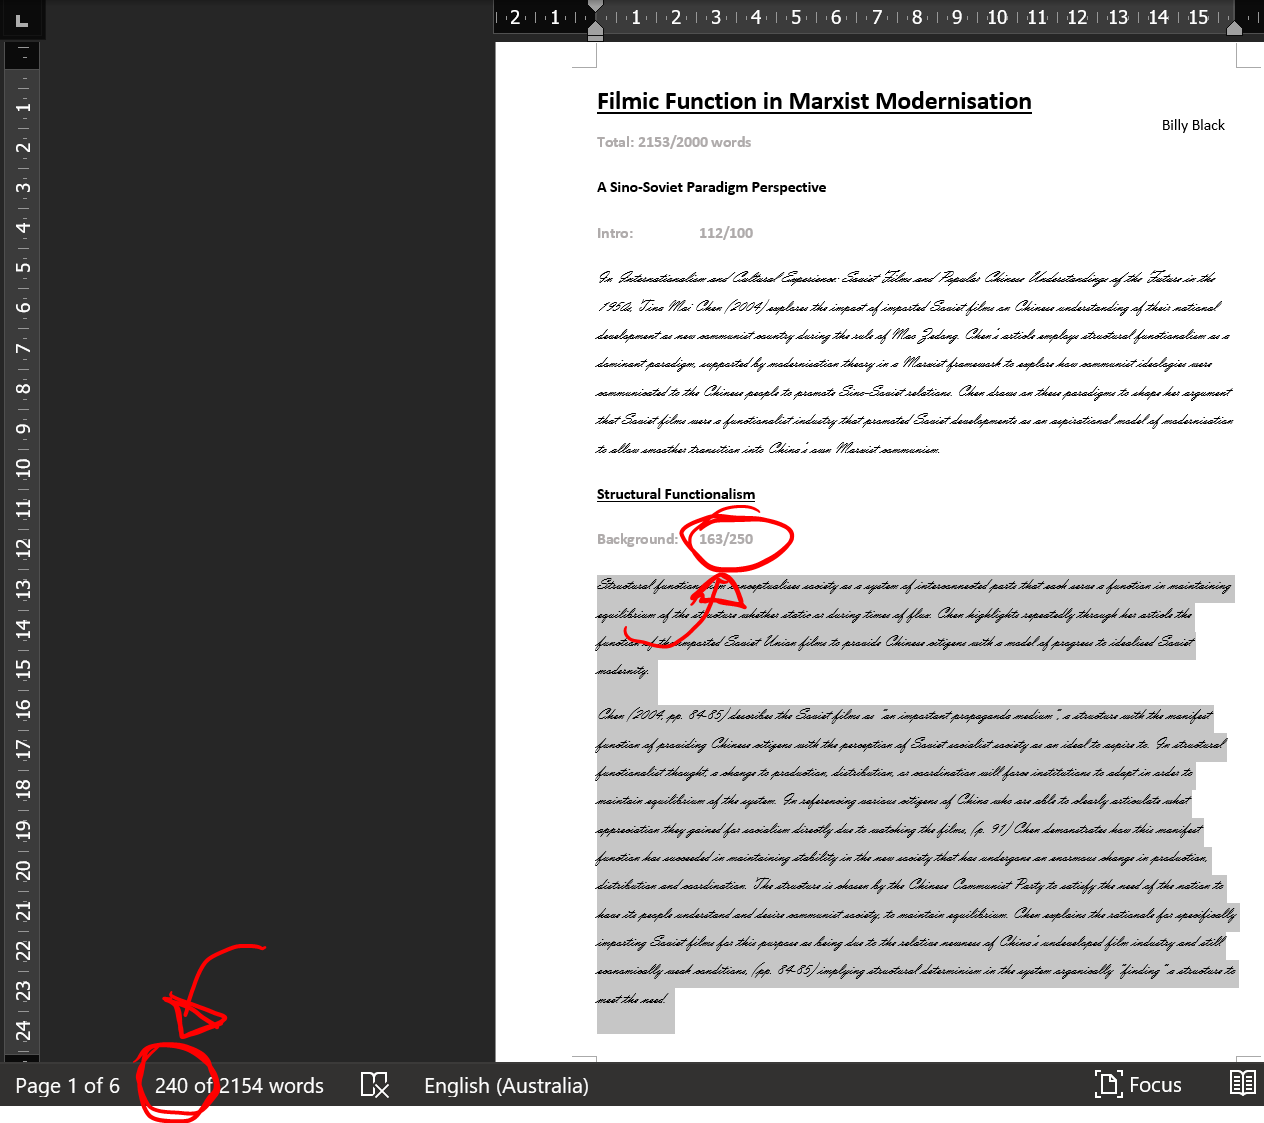
\includegraphics[scale=0.5]{figure/currentway.PNG}\\
\tiny{\textit{Screenshot of an attempt to manually track word count}}
    \end{column}
  \end{columns}

  
\end{frame}

%%%%%%%%%%%%%%%%%%%%%%%%%%%%%%%%%%%%%%%%%%%%%%%%%%%%%%%%%%%%%%%%%%%%%%%%%%
\mysection{line}
%%%%%%%%%%%%%%%%%%%%%%%%%%%%%%%%%%%%%%%%%%%%%%%%%%%%%%%%%%%%%%%%%%%%%%%%%%
\begin{frame}\label{\secvariable}
\begin{center}
  \vspace{-1cm}
  
  \begin{columns}[t]
  %https://tex.stackexchange.com/a/7452/5483
    \begin{column}[c]{0.5\textwidth}
    \parbox{\linewidth}{\small
    
    \vspace{2em}
    
\centering\textbf{\underline{What is chunking?}}\flushleft
    
    \vspace{1em}
    
    Chopping large blocks of information into manageable smaller chunks, or
    
    \vspace{0.5em}
    
    Pooling together many small items of information into themed groups to avoid overwhelming the reader
    
    \vspace{0.5em}    
    
    It's not just the reader that benefits! 
    
    \vspace{0.5em}
    
    Chunking your writing gives you
    
    \begin{itemize}
        \item better familiarity with your own research
        \item a clearer view of your own arguments
        \item a stronger position due to better argument cohesion
    \end{itemize}}  

    \end{column}
\begin{column}[c]{0.6\textwidth}
 \centering
 
 \vspace{1em}
 
 \tiny{\textit{Visualisation of chunking CC BY-SA \href{https://upload.wikimedia.org/wikipedia/commons/9/9c/2_Views_of_Chunking\_\%28Figure\_2\%29.jpg}{via Wikimedia Commons}}}
 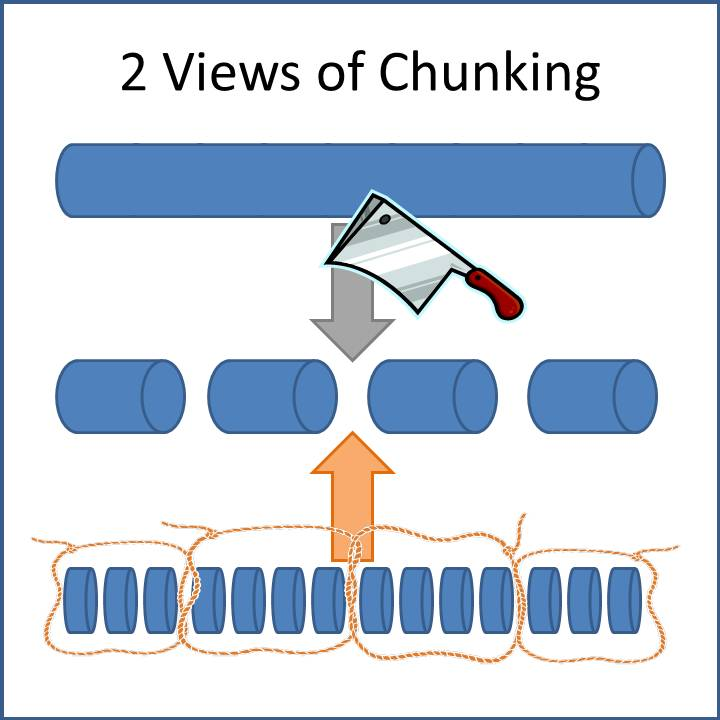
\includegraphics[width=1\textwidth,height=0.75\textheight,keepaspectratio]{%
  figure/chunking.jpg}
    
    \vspace{0.5em}
    \scriptsize Human short-term working memory functions best when only required to remember \textbf{3-4 items}!
    \end{column}
    
  \end{columns}

\end{center}
\end{frame}

%%%%%%%%%%%%%%%%%%%%%%%%%%%%%%%%%%%%%%%%%%%%%%%%%%%%%%%%%%%%%%%%%%%%%%%%%%
\mysection{major}
%%%%%%%%%%%%%%%%%%%%%%%%%%%%%%%%%%%%%%%%%%%%%%%%%%%%%%%%%%%%%%%%%%%%%%%%%%
\begin{frame}\label{\secvariable} %%Eine Folie
    \begin{columns}[t]
    %https://tex.stackexchange.com/a/7452/5483
    \begin{column}[c]{0.6\textwidth}
              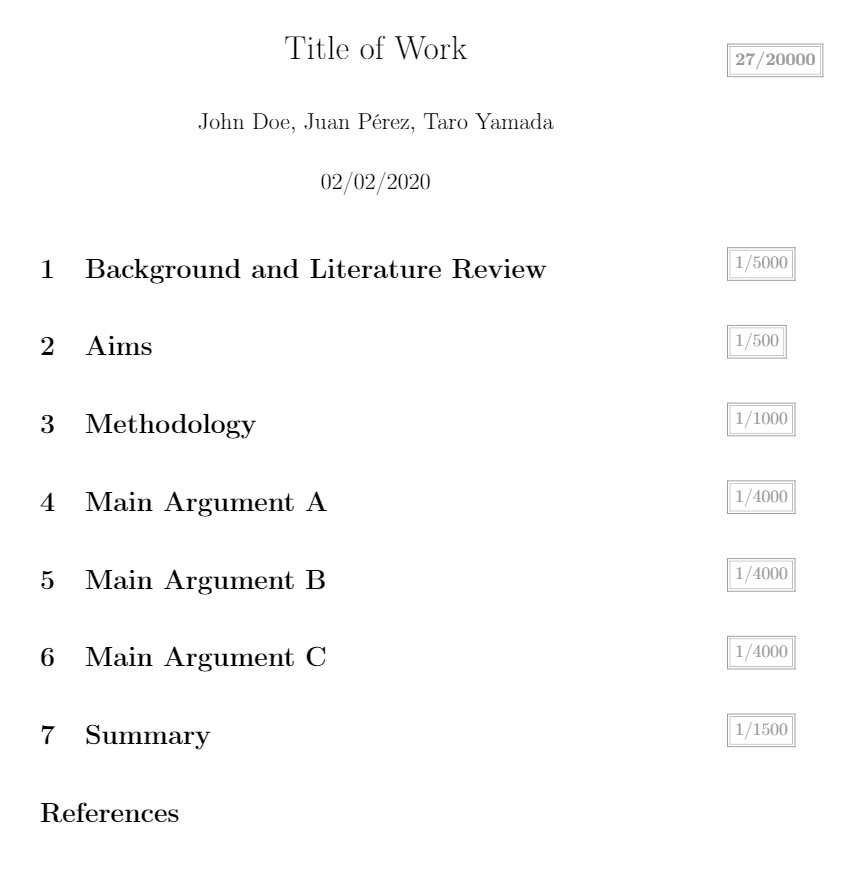
\includegraphics[scale=0.5]{figure/sectioning}
    
    \tiny{\textit{Screenshot of example of sectioning}} 
    \end{column}
    \begin{column}[c]{0.45\textwidth}
    \parbox{\linewidth}{

    \small An example of using chunking techniques with the focus frame to manage a 20 000 word research report.
    
    \vspace{12pt}
    
    Remembering to keep things in groups of 3-4, group the "research report sections" together, followed by the "main argument sections".
    
    \vspace{12pt}
    
    With word counts, we can already give weight to different sections and start planning what might go into a 4000 word main argument.      }
    \end{column}
    
  \end{columns}

    \parbox{\linewidth}{

}
\end{frame}


%%%%%%%%%%%%%%%%%%%%%%%%%%%%%%%%%%%%%%%%%%%%%%%%%%%%%%%%%%%%%%%%%%%%%%%%%%
\mysection{minor}
%%%%%%%%%%%%%%%%%%%%%%%%%%%%%%%%%%%%%%%%%%%%%%%%%%%%%%%%%%%%%%%%%%%%%%%%%%
\begin{frame}\label{\secvariable} %%Eine Folie
    \begin{columns}[t]
    %https://tex.stackexchange.com/a/7452/5483
    \begin{column}[c]{0.6\textwidth}
       \tiny{\textit{Screenshot of example of subsectioning}} 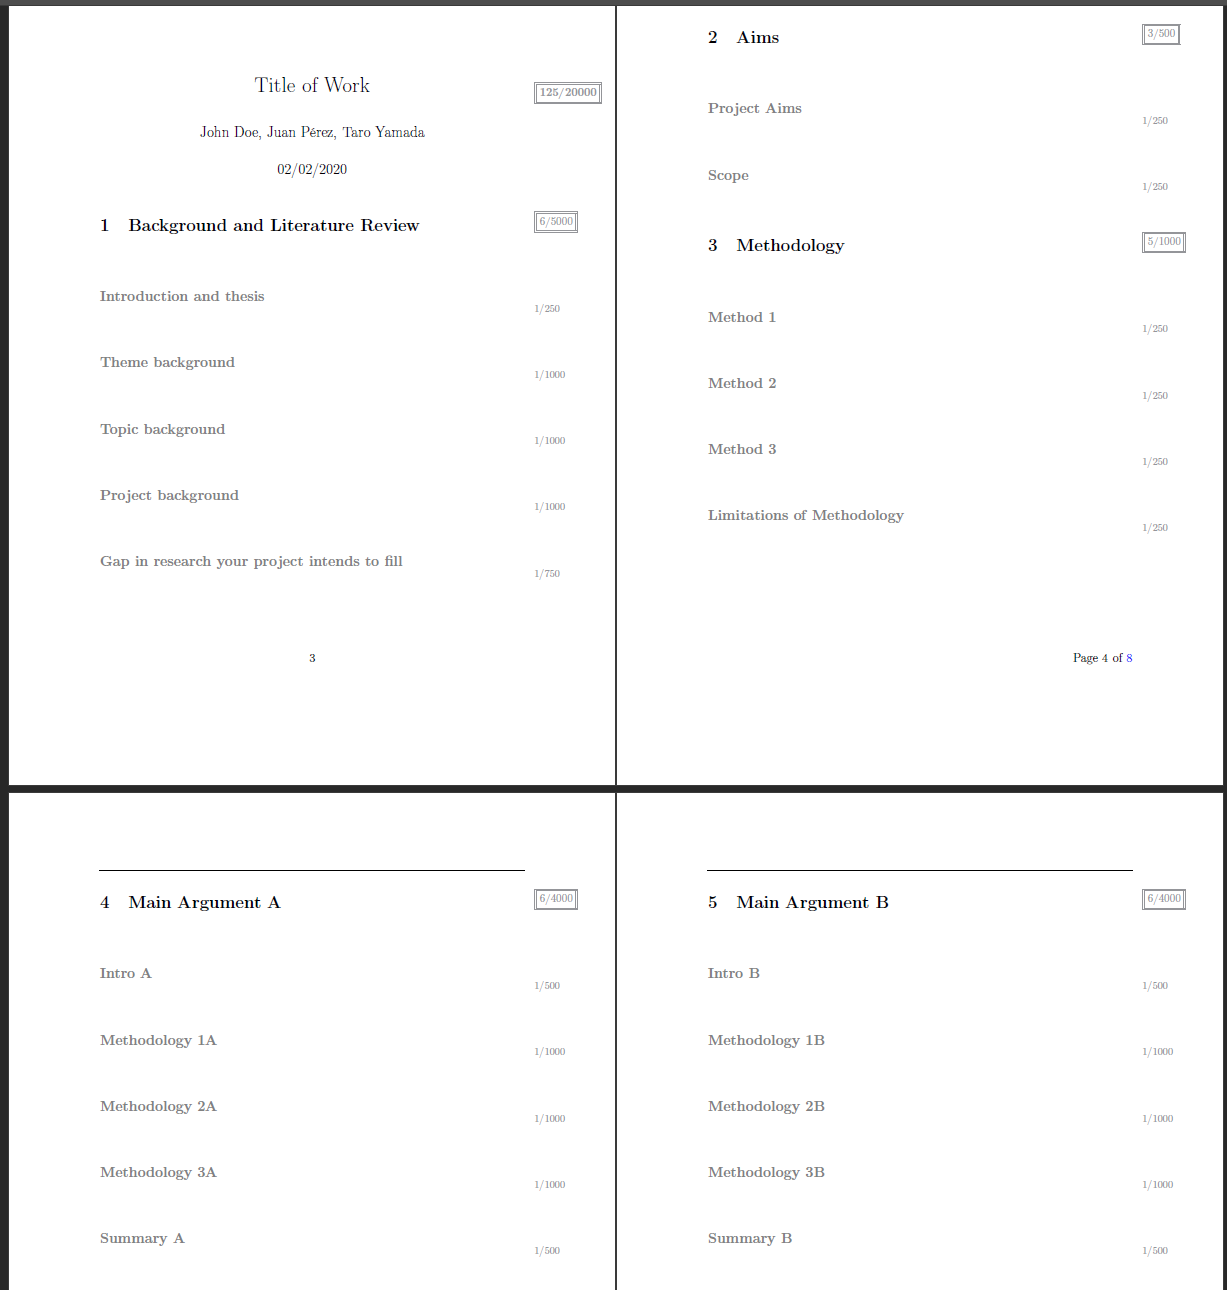
\includegraphics[scale=0.4]{figure/subsectioning}
    \end{column}
    \begin{column}[c]{0.45\textwidth}
    \parbox{\linewidth}{

    \small An example of using chunking techniques with the focus frame to manage a 20 000 word research report.
    
    \vspace{12pt}
    
    Now we have section length, we can plan what each section will comprise of.
    
    \vspace{12pt}
    
    Grouping subsections again into 3-4, divide up the word count into likely weighting.
    }
    \end{column}
    
  \end{columns}

\end{frame}

%%%%%%%%%%%%%%%%%%%%%%%%%%%%%%%%%%%%%%%%%%%%%%%%%%%%%%%%%%%%%%%%%%%%%%%%%%

%%%%%%%%%%%%%%%%%%%%%%%%%%%%%%%%%%%%%%%%%%%%%%%%%%%%%%%%%%%%%%%%%%%%%%%%%%
\begin{frame}\label{\secvariable}

\centering
\includegraphics[scale=0.55]{%
figure/readmeeg.PNG}

\tiny{\textit{Screenshot of demonstration of the focus frame}}  

\end{frame}

%%%%%%%%%%%%%%%%%%%%%%%%%%%%%%%%%%%%%%%%%%%%%%%%%%%%%%%%%%%%%%%%%%%%%%%%%%
\mysection{conclusion}
%%%%%%%%%%%%%%%%%%%%%%%%%%%%%%%%%%%%%%%%%%%%%%%%%%%%%%%%%%%%%%%%%%%%%%%%%%
\begin{frame}\label{\secvariable}
  
Full readme and style package available from \href{https://github.com/billyblacklington/focusframe}{github repository}

\vspace{12pt}

Available soon on \href{ctan.org}{CTAN: Comprehensive TeX Archive Network}

  
  
%   \usebeamerfont{bodytext}
%   K\"ohler, A., J. N. McElwaine, B. Sovilla, M. Ash, P. Brennan (in Review),
% Surge dynamics of the 3 February 2015 avalanches in Valle\'e de la Sionne,
% \textit{J. Geophys. Res.} 
  
\end{frame}



\end{document}
